\documentclass{article} % For LaTeX2e
\usepackage{nips12submit_e,times}
\usepackage{amsmath}
\usepackage{graphicx}
\usepackage{caption}
\usepackage{subcaption}
\usepackage{comment}
\usepackage[top=1.0in, bottom=1.0in, left=1.0in, right=1.0in]{geometry}

%\renewcommand\refname{Papers To Read}
\title{Semantic Segmentation Using Hybrid Markov Logic Networks}

\author{
Aravindh Mahendran \\
\texttt{amahend1@andrew.cmu.edu} \\ 
\And
Nitish Thatte \\
\texttt{nitisht@andrew.cmu.edu} \\
\AND
Adwait Gandhe \\
\texttt{agandhe@andrew.cmu.edu} \\
}

\newcommand{\fix}{\marginpar{FIX}}
\newcommand{\new}{\marginpar{NEW}}

\nipsfinalcopy

\begin{document}
\maketitle

\begin{abstract}
Semantic image segmentation is the process of assigning human relevant labels to pixels in an image and is a high level vision problem. Increasing the number of labels increases the complexity of the problem. Markov Logic Networks (MLNs) allow us to handle uncertainty and complexity in a single framework, whereas Hybrid Markov Logic Networks (HMLNs) are an extension of the MLNs that allow continuous properties and functions over those properties as features.  In this paper, we propose a method for semantic segmentation using Hybrid Markov Logic Networks, which integrate first order logic and statistical learning.  
\end{abstract}


\section{Introduction}
\label{sec:Intro}
Semantic segmentation is the process of assigning a class label to each pixel of the image. This is an important problem in computer vision for understanding the underlying information in an image. While classical segmentation techniques group together the pixels based on low level features, semantic segmentation adopts a supervised learning approach. There are two common approaches for semantic segmentation. The first makes use of low level features and combines them with a learning framework to obtain higher level labels. The second approach is to use low level cues, rather than features, with random fields and learn a unified framework using low level segmentation. In this paper we explore the second approach further by combining logical and statistical techniques to jointly address the issues of uncertainty and complexity. 

This paper is structured as follows: Section \ref{sec:Related} discusses the related work. In section \ref{sec:Attempt}, we discuss methods that we have attempted for semantic segmentation. The experiments conducted and the results obtained are presented in section \ref{sec:Exp}. Section \ref{sec:New} presents our approach for the second half of the semester. We summarize our conclusions in section \ref{sec:Conclusion}. And finally section \ref{sec:Plan} outlines our plan to implement the proposed approach.

%------------------------------------------------------------------------------------------

\section{Related Work}
\label{sec:Related}

One of the first approaches for simultaneous object segmentation and recognition utilizes an Implicit Shape Model that integrates both capabilities into a common probabilistic framework \cite{Leibe04combinedobject}. 
Another approach used a generative model based on the bag of words representation for such simultaneous recognition and segmentation \cite{cao:spatially}.  
Furthermore, a method based on some of these approaches for scoring low-level patches according to their class relevance and propagating these posterior probabilities to pixels has been developed \cite{conf/bmvc/CsurkaP08}.

Several recent approaches use random fields to incorporate local cues and impart global control without implementing low level segmentation. For example, \cite{Kumar:2005:OC:1068507.1068889} proposes a Bayesian method for combining top-down and bottom-up cues. Conditional random fields have also been used for this purpose \cite{Kumar:2005:HFF:1097115.1097790} \cite{Richard04multiscaleconditional}. Finally, Textonboost \cite{Shotton06textonboost:joint} is an approach to learning a discriminative model of object classes incorporating appearance, shape and context information efficiently. We suggest \cite{SegmentRegionsParts} for other semantic image segmentation approaches.

These approaches handle the complexity and uncertainty inherent in the structured inference problem in different ways. An alternate approach is to use Markov Logic Networks \cite{Domingos06unifyinglogical} \cite{Richardson06markovlogic} that attach weights to first-order formulae and view them as templates for building Markov Networks. Hybrid Markov Logic Networks (HMLNs)\cite{Wang_hybridmarkov} are an extension that allow for continuous properties to appear as features. In this paper we discuss our attempts to use HMLNs for semantic segmentation. 
\label{sec:Geo}
A recent approach for semantic segmentation is to use a learned label transfer confidence function to propagate labels between neighboring superpixels based on the geodesic distance metric \cite{Chen2012}. Labels are iteratively propagated across edges of a graph of connected superpixels based on geodesic distance.
\label{sec:RandFor}
Another recent approach \cite{IterContFor12} learns a single random forest and incrementally adds context features derived from coarser levels. Unlike Textonboost \cite{Shotton06textonboost:joint}, which learns two random forests, this approach models the dependencies between contextual and non-contextual features directly. 
\label{sec:bagofwords}
Semantic image segmentation has also been approached using the bag of words model. In one of the recent approaches, \cite{visualdictrene}, the authors develop a conditional random field model that combines dictionary learning, feature categorization (assigning key points to visual words) and image semantic segmentation into one framework.
%------------------------------------------------------------------------------------------

\section{Attempted Methods}
\label{sec:Attempt}
%------------------------------------------------------------------------------------------
\subsection{Label Propagation}
\label{sec:AttemptLabProp}

	In section \ref{sec:Geo}, we discussed a method of propagating labels on a graph of connected superpixels based on a learned label transfer confidence function. This method introduced us to two ideas: propagating labels rather than directly minimizing a cost function to arrive at a segmentation and working with graphs of related superpixels. Building on these ideas, we learn the weights for a hybrid Markov logic network in order to refine a prior expected segmentation obtained from a baseline algorithm. The method incorporates an undirected graph of connected superpixels that expresses where labels can propagate.

%TODO
	Using a MLN provides several advantages. First, MLNs allows us to perform metric learning by discovering a different weight for every label and feature vector component combination. Therefore, an MLN can model complex systems more easily than an SVM or logistic regression, which can learn one weight vector for all labels. Another advantage of MLNs is that they allow the user to express a template for his or her model using first order logic, a language that is easy to understand and learn.

Definition of Markov logic network: Numeric terms and predicates:
\begin{align*}
	\mathrm{featureDistance}(s_i,s_j,f_m) & \quad \textrm{Numeric term equal to the distance based on the $m^\textrm{th}$ component of feature vectors} \\
		& \quad \textrm{for superpixels $s_i$ and $s_j$.} \\
	\mathrm{isLabel}(s_i,l_k) &\quad \textrm{Boolean predicate, True if $s_i$ is assigned label $l_k$, false otherwise.} \\
	\mathrm{isNeighbor}(s_i,s_j) & \quad \textrm{Boolean predicate, True if $s_i$ and $s_j$ are neighbors in our superpixel connectivity graph.}
\end{align*}

Formulae:
\begin{align*}
	\mathrm{isNeighbor}(s_i,s_j) &\Rightarrow (\mathrm{isLabel}(s_i,l_k) \Leftrightarrow \mathrm{isLabel}(s_k,l_m)) \\
	(\mathrm{isLabel}(s_i,l_k) &\Leftrightarrow \mathrm{isLabel}(s_k,l_m)) \times \mathrm{featureDistance}(s_i, s_k, f_m)
\end{align*}

These formulae encode that Superpixels with similar feature vectors should have the same label and superpixels that are connected by an edge (are neighbors) should also have the same label.

A brute-force approach to this problem would be to allow every superpixel to transfer its label to every other superpixel. Such a graph would allow superpixel labels to be learned from a more global context in the image. However, this would overly complicate the underlying Markov random field, thus making learning and inference intractable. In contrast, a simple approach is to connect nodes that are directly share borders. This approach, however, would only use local context for label propagation.

Therefore, we propose to take a middle ground approach that will produce densely connected superpixels where relations are expected to be strong, and fewer edges across boundaries expected not to share labels. In order to build this superpixel graph, we take two levels of superpixel segmentations: A coarse level, which we will henceforth refer to as supersuperpixels, and a fine level, which we term superpixels. These segmentations were found using the algorithm outlined in \cite{Superpixel}. All superpixels within a supersuperpixel are connected allowing for contextual information to be shared within a region. Additionally, superpixels that share a boundary between two supersuperpixels are connected allowing for labels to propagate across supersuperpixels while acknowledging that label transfer across these borders is less probable than within a supersuperpixel. We then search through the training data set and select the $k-$Nearest Neighbors based on euclidean distance between GIST features \cite{Gist} of the images. We use the superpixels in these $k$ images to train the MLN on the formulae listed above.

\subsection{Other Approaches}
\label{sec:IterContFor}
We attempted to learn a HMLN on an ensemble of feature sets such as those used by \cite{IterContFor12}. In spite of the advantages of this approach, the HMLN does not afford the use of a large number of features the way random forests do. Hence we abandoned this approach. 
\label{sec:BofWordApp}
Even though the bag of words approach developed in \cite{visualdictrene} has shown very good results on the CAMVID\cite{BrostowFC:PRL2008} and Graz-02 \cite{graz02} datasets, it cannot be incorporated into a MLN as it requires second order logic. Particularly, the word count histogram built as part of the bag of words model requires a count of the number of true predicates of a certain kind which is a meta level information beyond the first order logic. Hence, we abandoned this approach.

\section{Experiment}
\label{sec:Exp}

We used the Alchemy - Open Source AI software \cite{alchemy} for learning the weights for the HMLN. Results described in this section are from the MSRC v1 dataset \cite{DBLP:conf/iccv/WinnCM05}. The 3 nearest neighbors from the training set of a query image are retrieved. Superpixels (fine and coarse, ~1000 and ~40 superpixels respectively), adjacency matrices and word maps are computed for each image. These are illustrated in \ref{fig:labelprop:preprocess}. An initial baseline segmentation for the test image is computed by matching bag of words histograms of individual superpixels to histograms from the training set. The $28-$nearest histograms based on euclidean distance were retrieved and a probability vector was computed based on the counts of individual labels in this collection.
Unfortunately, we ran into memory issues with the system using more than 23 Gb of virtual memory forcing it to kill the process. 

\begin{figure}
	\centering
	\begin{comment}
		\begin{subfigure}[c]{\textwidth}
			\centering
			\begin{subfigure}[c]{0.195\textwidth}
				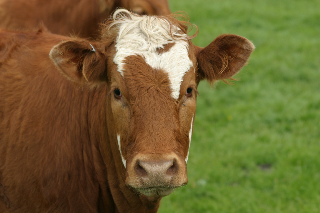
\includegraphics[width = \textwidth]{./img/1_22_s.png}
				\label{fig:1_22_s}
			\end{subfigure}
			\begin{subfigure}[c]{0.195\textwidth}
				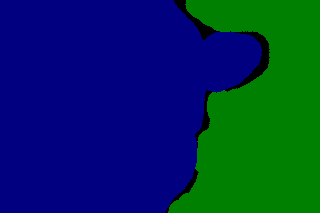
\includegraphics[width = \textwidth]{./img/1_22_s_GT.png}
				\label{fig:1_22_s_lab}
			\end{subfigure}
			\begin{subfigure}[c]{0.195\textwidth}
				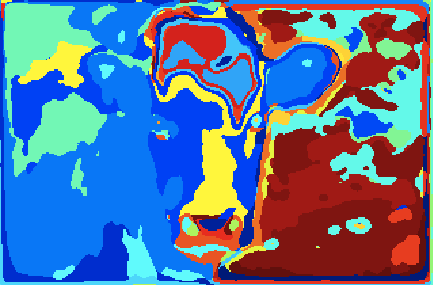
\includegraphics[width = \textwidth]{./img/1_22_s_map.png}
				\label{fig:1_22_s_map}
			\end{subfigure}
			\begin{subfigure}[]{0.195\textwidth}
				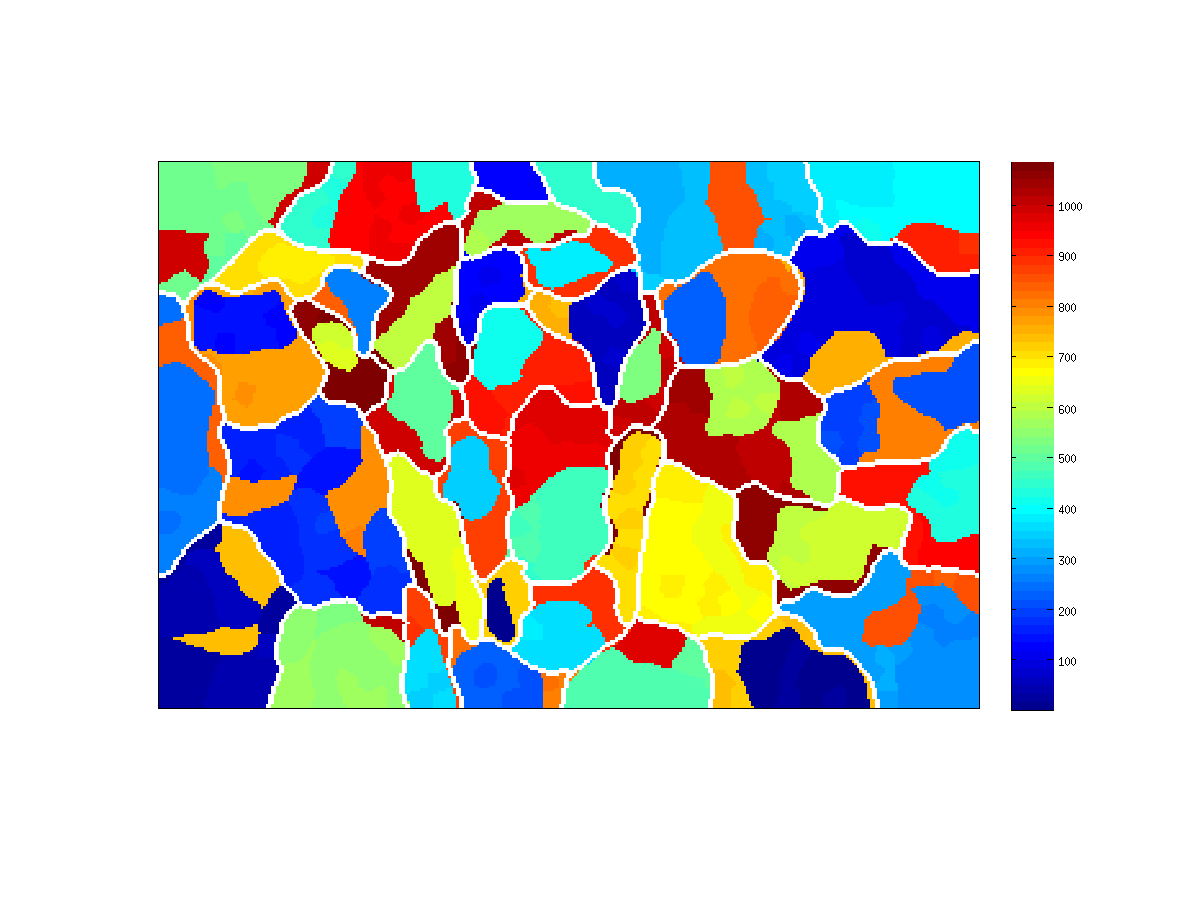
\includegraphics[width = \textwidth]{./img/su1_22_s.pdf}
				\label{fig:1_22_s_su}
			\end{subfigure}
			\begin{subfigure}[c]{0.195\textwidth}
				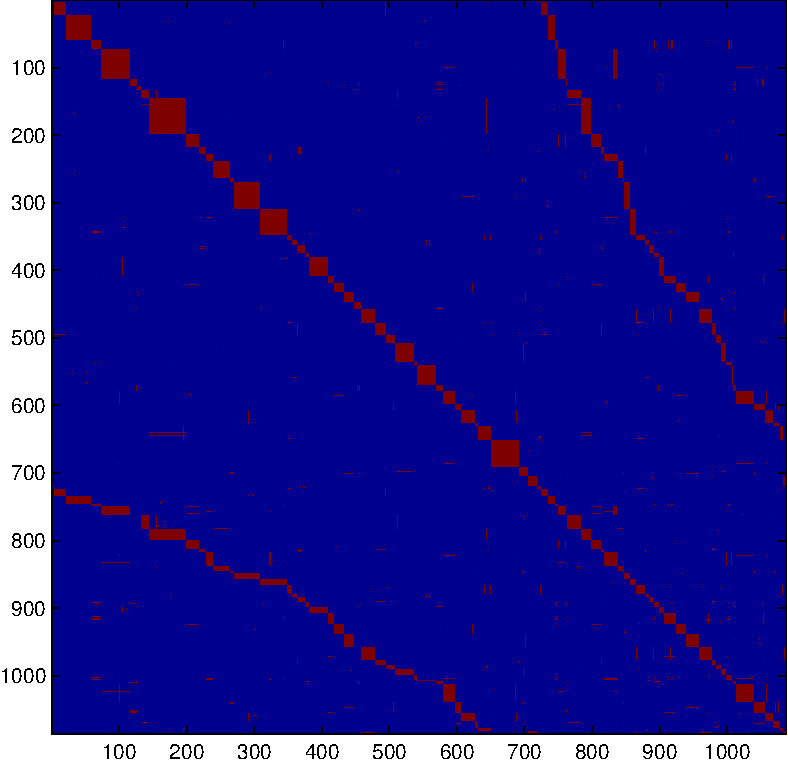
\includegraphics[width = \textwidth]{./img/adj1_22_s.pdf}
				\label{fig1_22_s_adj}
			\end{subfigure}
		\end{subfigure}

	\begin{subfigure}[c]{\textwidth}
		\centering
		\begin{subfigure}[c]{0.195\textwidth}
			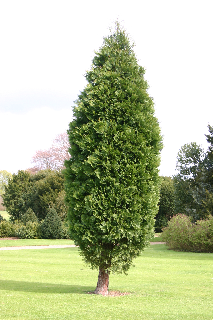
\includegraphics[width = \textwidth]{./img/2_21_s.png}
			\label{fig:2_21_s}
		\end{subfigure}
		\begin{subfigure}[c]{0.195\textwidth}
			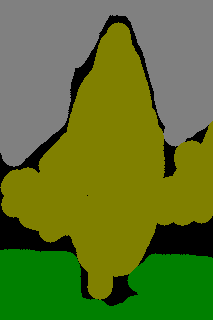
\includegraphics[width = \textwidth]{./img/2_21_s_GT.png}
			\label{fig:2_21_s_lab}
		\end{subfigure}
		\begin{subfigure}[c]{0.195\textwidth}
			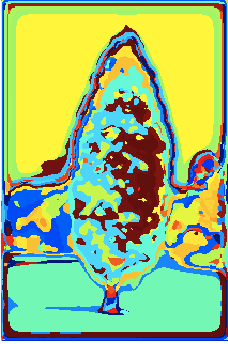
\includegraphics[width = \textwidth]{./img/2_21_s_map.png}
			\label{fig:2_21_s_map}
		\end{subfigure}
		\begin{subfigure}[]{0.195\textwidth}
			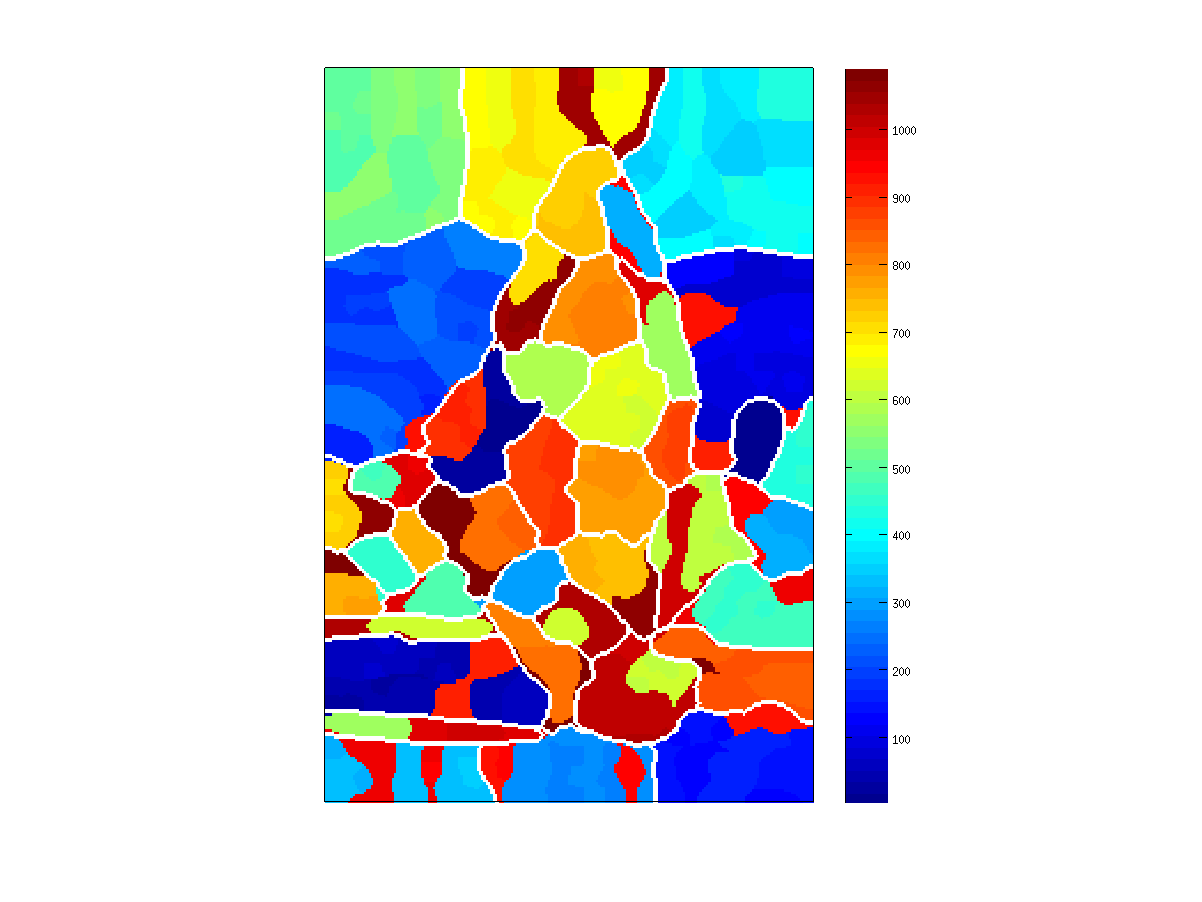
\includegraphics[width = \textwidth]{./img/su2_21_s.pdf}
			\label{fig:2_21_s_su}
		\end{subfigure}
		\begin{subfigure}[c]{0.195\textwidth}
			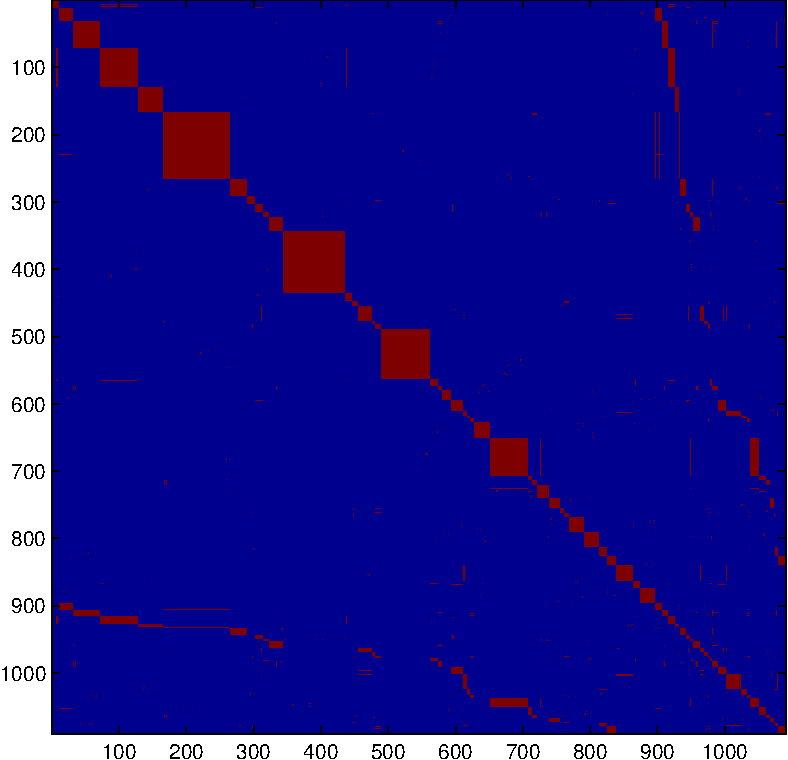
\includegraphics[width = \textwidth]{./img/adj2_21_s.pdf}
			\label{fig2_21_s_adj}
		\end{subfigure}
	\end{subfigure}
	\end{comment}
	\begin{subfigure}[c]{\textwidth}
		\centering
		\begin{subfigure}[c]{0.195\textwidth}
			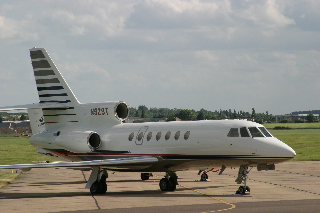
\includegraphics[width = \textwidth]{./img/4_1_s.png}
			\label{fig:4_1_s}
		\end{subfigure}
		\begin{subfigure}[c]{0.195\textwidth}
			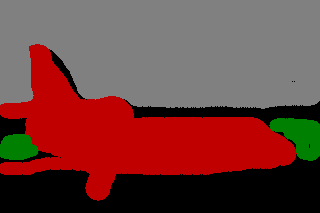
\includegraphics[width = \textwidth]{./img/4_1_s_GT.png}
			\label{fig:4_1_s_lab}
		\end{subfigure}
		\begin{subfigure}[c]{0.195\textwidth}
			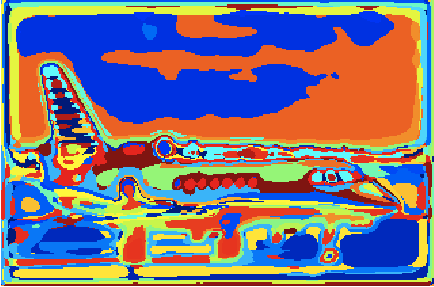
\includegraphics[width = \textwidth]{./img/4_1_s_map.png}
			\label{fig:4_1_s_map}
		\end{subfigure}
		\begin{subfigure}[]{0.195\textwidth}
			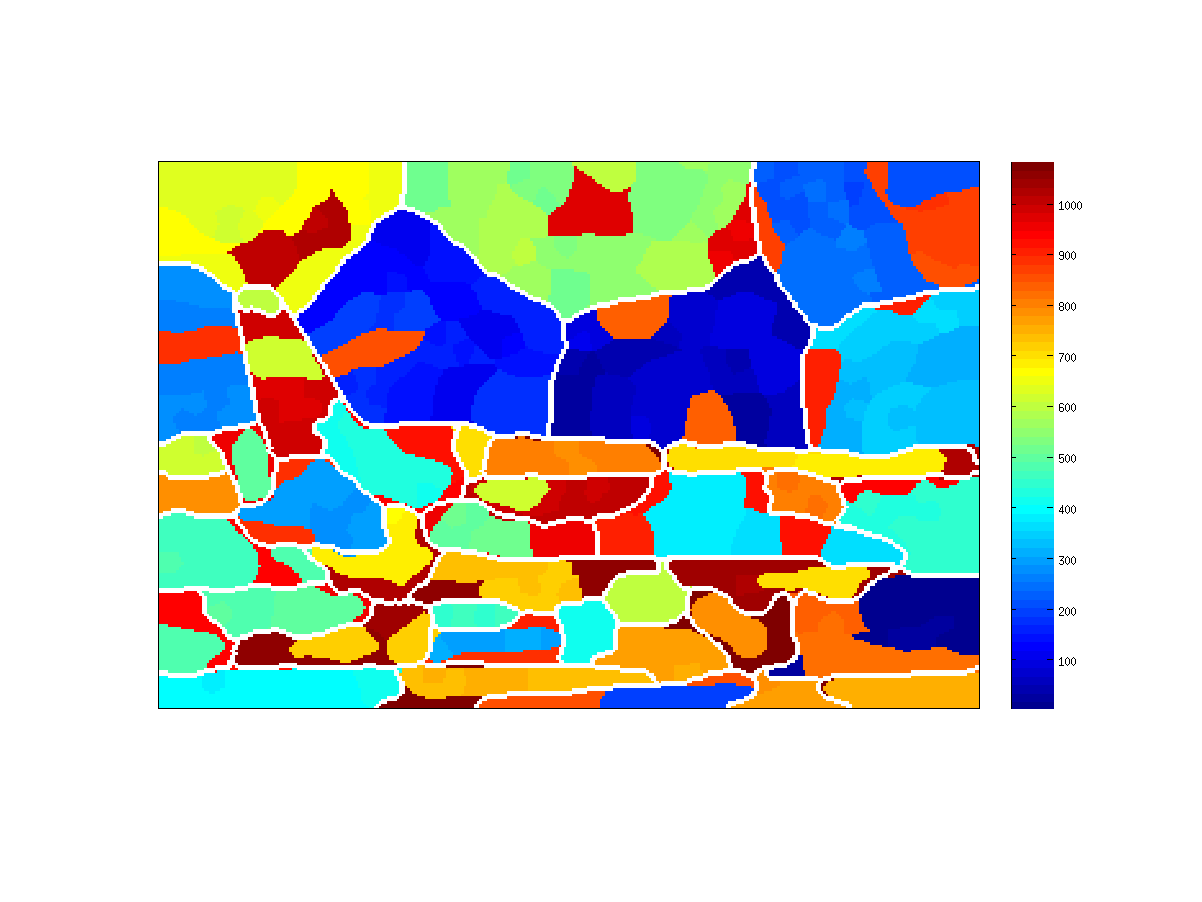
\includegraphics[width = \textwidth]{./img/su4_1_s.pdf}
			\label{fig:4_1_s_su}
		\end{subfigure}
		\begin{subfigure}[c]{0.195\textwidth}
			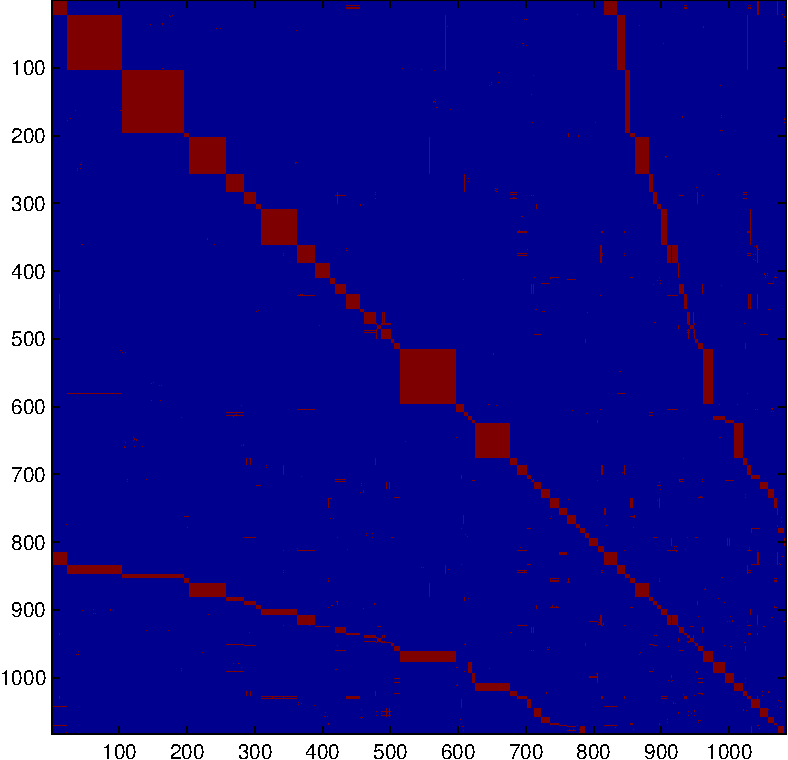
\includegraphics[width = \textwidth]{./img/adj4_1_s.pdf}
			\label{fig4_1_s_adj}
		\end{subfigure}
	\end{subfigure}
	
	\begin{comment}
		\begin{subfigure}[c]{\textwidth}
			\centering
			\begin{subfigure}[c]{0.195\textwidth}
				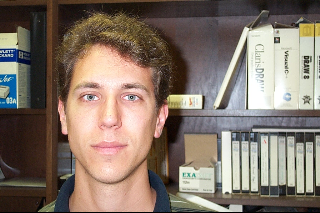
\includegraphics[width = \textwidth]{./img/6_3_s.png}
				\label{fig:6_3_s}
			\end{subfigure}
			\begin{subfigure}[c]{0.195\textwidth}
				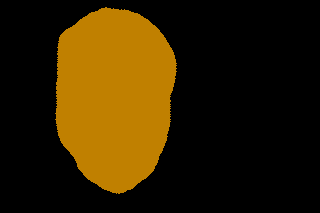
\includegraphics[width = \textwidth]{./img/6_3_s_GT.png}
				\label{fig:6_3_s_lab}
			\end{subfigure}
			\begin{subfigure}[c]{0.195\textwidth}
				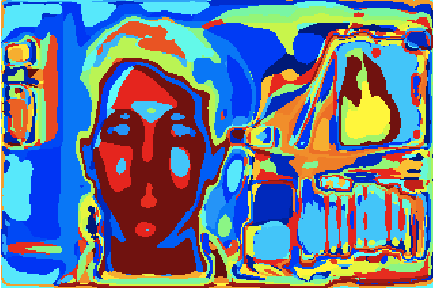
\includegraphics[width = \textwidth]{./img/6_3_s_map.png}
				\label{fig:6_3_s_map}
			\end{subfigure}
			\begin{subfigure}[]{0.195\textwidth}
				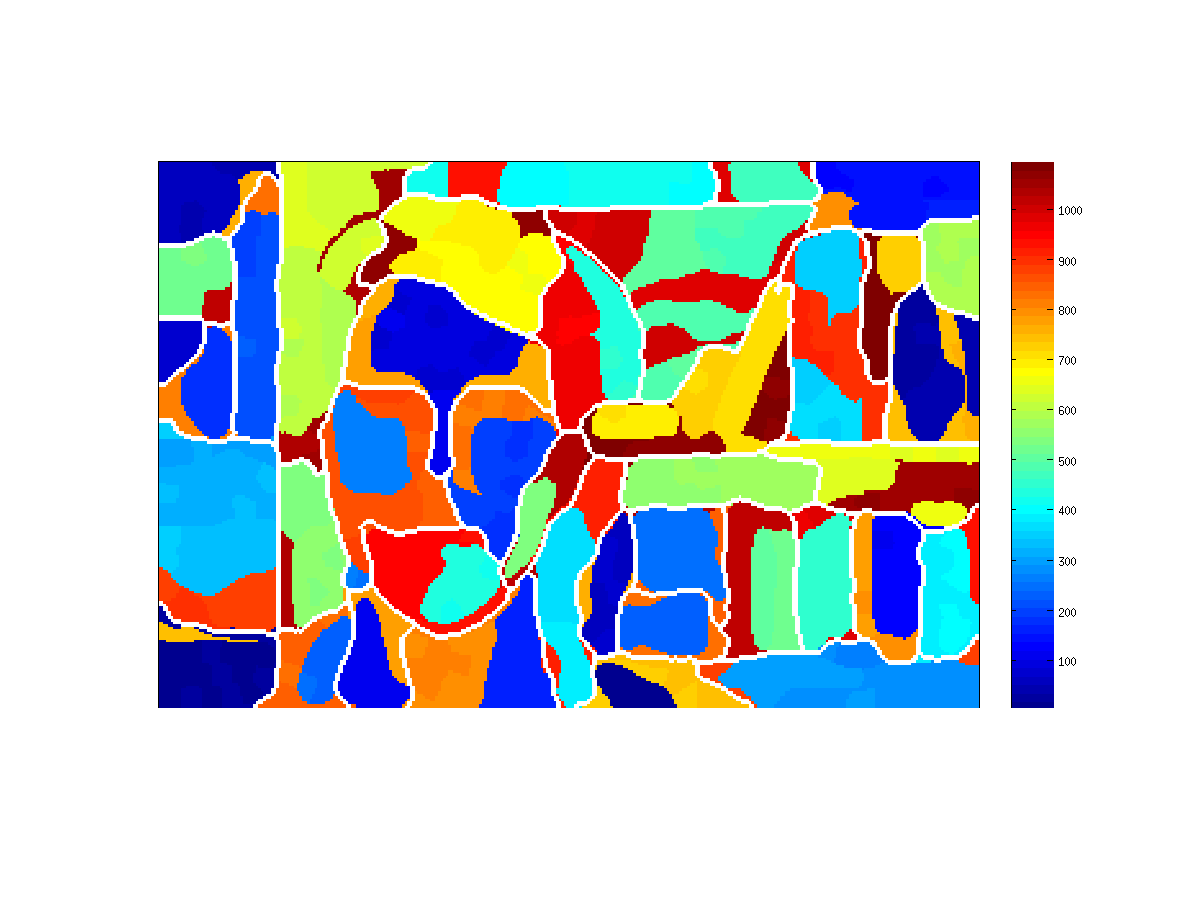
\includegraphics[width = \textwidth]{./img/su6_3_s.pdf}
				\label{fig:6_3_s_su}
			\end{subfigure}
			\begin{subfigure}[c]{0.195\textwidth}
				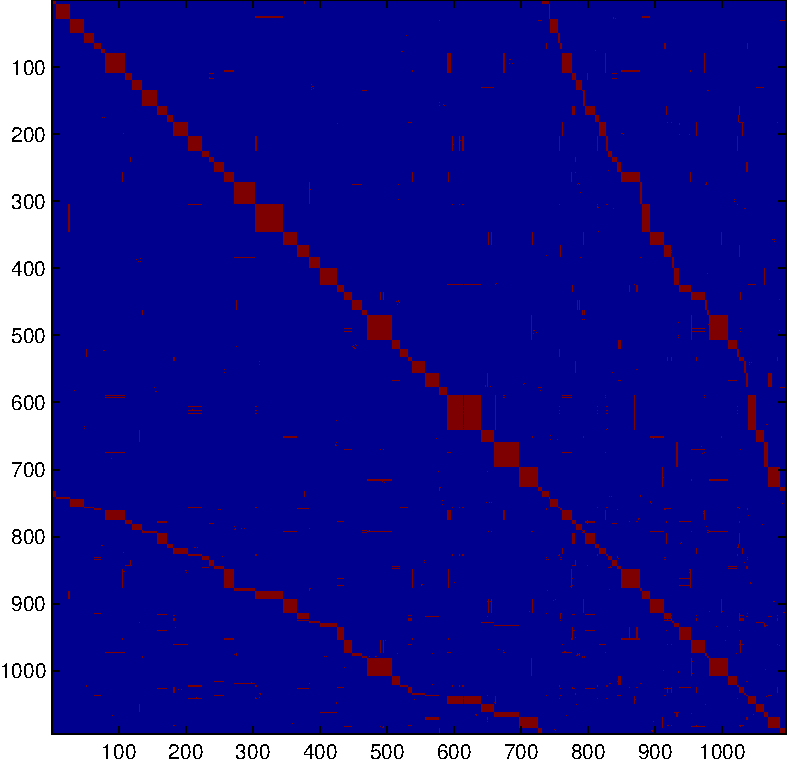
\includegraphics[width = \textwidth]{./img/adj6_3_s.pdf}
				\label{fig6_3_s_adj}
			\end{subfigure}
		\end{subfigure}

		\begin{subfigure}[c]{\textwidth}
			\centering
			\begin{subfigure}[c]{0.195\textwidth}
				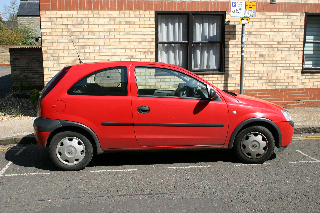
\includegraphics[width = \textwidth]{./img/7_8_s.png}
				\label{fig:7_8_s}

			\end{subfigure}
			\begin{subfigure}[c]{0.195\textwidth}
				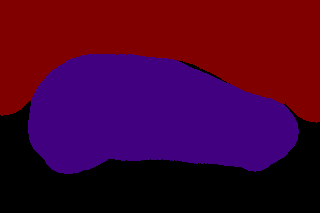
\includegraphics[width = \textwidth]{./img/7_8_s_GT.png}
				\label{fig:7_8_s_lab}
			\end{subfigure}
			\begin{subfigure}[c]{0.195\textwidth}
				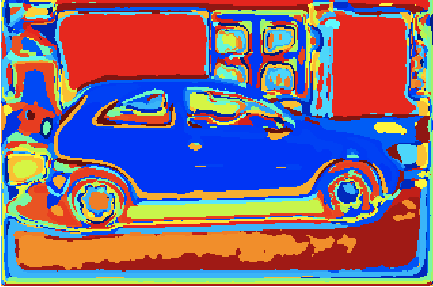
\includegraphics[width = \textwidth]{./img/7_8_s_map.png}
				\label{fig:7_8_s_map}
			\end{subfigure}
			\begin{subfigure}[]{0.195\textwidth}
				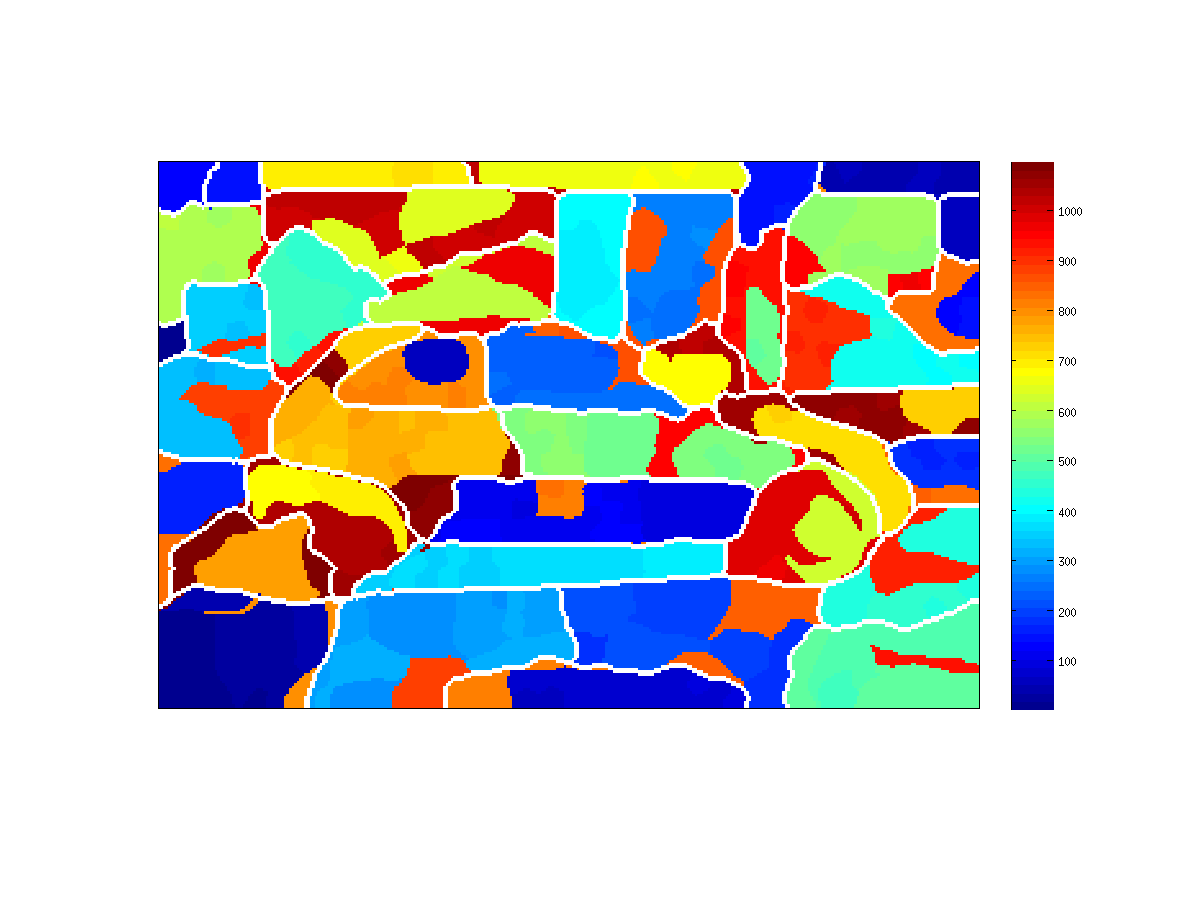
\includegraphics[width = \textwidth]{./img/su7_8_s.pdf}
				\label{fig:7_8_s_su}
			\end{subfigure}
			\begin{subfigure}[c]{0.195\textwidth}
				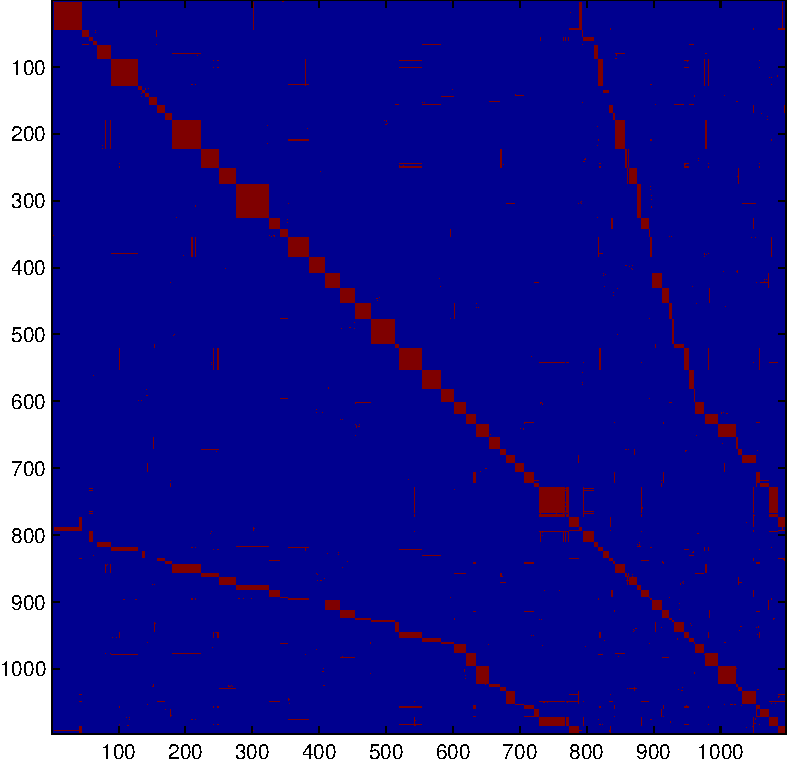
\includegraphics[width = \textwidth]{./img/adj7_8_s.pdf}
				\label{fig7_8_s_adj}
			\end{subfigure}
		\end{subfigure}

	\end{comment}	
	\begin{subfigure}[t]{\textwidth}
		\centering
		\begin{subfigure}[t]{0.195\textwidth}
			\subcaption{original image}
		\end{subfigure}
		\begin{subfigure}[t]{0.195\textwidth}
			\subcaption{ground truth segmentation}
		\end{subfigure}
		\begin{subfigure}[t]{0.195\textwidth}
			\subcaption{visual words map}
		\end{subfigure}
		\begin{subfigure}[t]{0.195\textwidth}
			\subcaption{superpixel segmentation}
		\end{subfigure}
		\begin{subfigure}[t]{0.195\textwidth}
			\subcaption{superpixel adjacency matrix}
		\end{subfigure}
	\end{subfigure}
	\caption{Pre-processing pipeline for label propagation experiment.}
	\label{fig:labelprop:preprocess}
	
\end{figure}
%------------------------------------------------------------------------------------------
\section{New Proposed Method}
\label{sec:New}
After attempting such varied methods using Markov logic networks, we realize that Markov logic is not a good solution to problems in low level vision due to combinatorial explosion. Therefore, we propose to use Markov logic for high level reasoning only. We consider all possible outputs of a meanshift based unsupervised segmentation algorithm by varying the parameters involved and use Markov logic to choose the best of these predictions. We generate a random set of parameter values for the unsupervised segmentation algorithm. An SVM classifier is trained to predict the label for each segment. Each such semantic segmentation corresponds to a parse of the image. An HMLN associates a consistency value with a given parse which evaluates the initial segmentation and classifier output. We choose the best current parameter settings and repeat this process by generating another random set of parameters within the neighborhood of the current values.  

Following the implementation of this approach, we shall experiment on the CAMVID dataset. This dataset consists of 4 video sequences. In the first set of experiments, we shall train on a random subset of frames in each video and test the trained model on the remaining frames of that video itself. The split would be 50:50. Parameters, specifically the window size and sample resolution for meanshift parameter generation, will be derived using cross validation. A second set of experiments would train the model on one video sequence and test it on the other three.

%------------------------------------------------------------------------------------------

\section{Conclusion}
\label{sec:Conclusion}

As mentioned in the project proposal, we have attempted to model different approaches for semantic image segmentation using HMLNs. We further analyzed why these are infeasible and proposed a new method for addressing the problem.

%------------------------------------------------------------------------------------------\bibliography{midway_report}
\bibliographystyle{plain}
\bibliography{midway_report}
%------------------------------------------------------------------------------------------\bibliography{midway_report}

\appendix
\section{Plan of Activities}
\label{sec:Plan}
\subsection*{Old Plan of Activities}
From now until the midterm report, Nitish will work on writing HMLNs, Aravindh will work on feature extraction and Adwait will work on super-pixel generation techniques. The midterm report will consist of the results of initial experiments with different techniques for each aspect and present our design choices.
\subsection*{New Plan of Activities}
Work so far suggest a radical change in approach. Aravindh will work on meanshift segmentation and understand its parameter space. Nitish and Adwait will work on building HMLNs for tree parsing and consistency evaluation.
\end{document}
